\documentclass[11pt,a4paper]{article}
\usepackage[utf8]{inputenc}
\usepackage[T1]{fontenc}
\usepackage[brazilian]{babel}
\usepackage{amsmath,amssymb,amsthm,mathtools}
\usepackage{icomma}
\usepackage{booktabs,longtable,array}
\usepackage{graphicx}
\usepackage[a4paper,margin=2.3cm]{geometry}
\usepackage[hidelinks]{hyperref}
\usepackage{float}
\usepackage[font=small,labelfont=bf,skip=4pt]{caption}
\newcommand{\bh}{\mathbf{h}}\newcommand{\bW}{\mathbf{W}}\newcommand{\bb}{\mathbf{b}}\newcommand{\bc}{\mathbf{c}}
\newcommand{\bP}{\mathbf{P}}\newcommand{\bF}{\mathbf{F}}\newcommand{\bFt}{\widetilde{\mathbf{F}}}\newcommand{\bQ}{\mathbf{Q}}
\newcommand{\bM}{\mathbf{M}}\newcommand{\bD}{\mathbf{D}}\newcommand{\bT}{\mathbf{T}}\newcommand{\bS}{\mathbf{S}}
\newcommand{\bR}{\mathbf{R}}\newcommand{\byh}{\hat{\mathbf{y}}}\newcommand{\bX}{\mathbf{X}}
\newcommand{\thT}{\boldsymbol{\theta}_T}\newcommand{\thS}{\boldsymbol{\theta}_S}\newcommand{\bu}{\mathbf{u}}
\newcommand{\bI}{\mathbf{I}}\newcommand{\R}{\mathbb{R}}\newcommand{\En}{\mathcal{E}}
\DeclareMathOperator{\sen}{sen}
\setlength{\emergencystretch}{3em}\setlength{\parindent}{0pt}\setlength{\parskip}{6pt}
\title{Neural Fourier Head: um exemplo sintético passo a passo,\\com todas as contas à mão}
\author{Experimento \texttt{exemplo\_sintetico} da rodada de 21/11/2026}
\date{}
\begin{document}
\maketitle


\section*{Resultado da confirmação (leia primeiro)}

Este exemplo foi construído para mostrar a Neural Fourier Head (NFH) \textbf{num caso favorável e pré-registrado} (regra e critério fixados por escrito antes de rodar). Isso \textbf{não é uma regra geral}: em dados reais da dissertação, a NFH treinada do zero perdeu da camada densa. Aqui, a combinação foi escolhida só pela validação (sementes 0 a 4) e depois reavaliada no teste com as sementes 10 a 19, que não participaram da seleção. Essas sementes mudam só a inicialização dos pesos e a ordem dos lotes de treino: \textbf{a série e as janelas de teste são as mesmas} da seleção e do teste de exemplificação de 16/11 (mesma semente de dados 2026, $N=9000$, cortes $60\,\%$ e $80\,\%$). Por isso o resultado mostra estabilidade entre inicializações, e não um resultado em dados novos. Em cada par ``média $\pm$ desvio'' abaixo, o $\pm$ é o desvio-padrão amostral (denominador $n-1$) entre as 10 sementes, e todos os valores têm quatro casas decimais. RMSE é a raiz do erro quadrático médio das previsões e MAE é o erro absoluto médio, ambos na escala do alvo; menor é melhor. Os números da confirmação estão na Tabela~\ref{tab:prim}. O RMSE de teste da NFH fica $2,6\,\%$ acima do RMSE do oráculo ($0,2961$, a referência amostral das mesmas janelas de teste) e o da camada densa (cabeça linear comum, que escreve direto os valores do horizonte previsto), $11\,\%$ acima. A densa+E é a densa treinada por mais $E=50$ épocas (a T1 usa outro $E$; ver Seção~\ref{sec:modelo}). A NFH teve RMSE menor que a densa em 10 das 10 sementes e menor que a densa+E em 10; no MAE, 10 e 10. O critério pré-registrado (médias de RMSE e de MAE da NFH menores ou iguais às da densa e às da densa+E, e RMSE menor que o da densa+E em pelo menos 8 sementes) foi \textbf{cumprido: veredito SUCESSO}. O modelo é pequeno: o backbone (a parte que lê a janela) tem uma camada com $p=16$ neurônios e 1040 parâmetros, e a cabeça tem mais 136, nas duas variantes, para que todas as contas caibam nas páginas seguintes.

\begin{table}[H]
\centering
\caption{Confirmação no teste: média $\pm$ desvio-padrão amostral entre as 10 sementes (menor é melhor). As duas últimas colunas contam em quantas sementes a NFH tem erro estritamente menor que o da variante da linha (RMSE e MAE). A última linha é um controle relatado depois da confirmação e não entra no critério (Seção~\ref{sec:resumo}).}\label{tab:prim}
\footnotesize
\resizebox{\textwidth}{!}{%
\begin{tabular}{lcccc}
\toprule
variante & RMSE de teste & MAE de teste & NFH menor (RMSE) & NFH menor (MAE) \\
\midrule
NFH (\emph{zero\_L1000}) & $0,3038$ $\pm$ $0,0015$ & $0,2445$ $\pm$ $0,0011$ & -- & -- \\
camada densa & $0,3282$ $\pm$ $0,0116$ & $0,2625$ $\pm$ $0,0088$ & 10/10 & 10/10 \\
densa+E & $0,3285$ $\pm$ $0,0124$ & $0,2625$ $\pm$ $0,0093$ & 10/10 & 10/10 \\
densa projetada em $\bT\oplus\bS$ (controle) & $0,3276$ $\pm$ $0,0115$ & $0,2621$ $\pm$ $0,0087$ & 10/10 & 10/10 \\
\bottomrule
\end{tabular}
}
\par\vspace{2pt}{\footnotesize Fonte: elaborado pelo autor; \texttt{confirmacao.csv} e \texttt{projecao\_confirmacao.csv}.}
\end{table}

O passo a passo usa a semente 10 (a primeira da confirmação): nela, RMSE e MAE de teste são $0,3039$ e $0,2447$ para a NFH, $0,3399$ e $0,2719$ para a densa e $0,3365$ e $0,2686$ para a densa+E. O retreino determinístico reproduziu esses valores (diferença máxima $5,6\times 10^{-17}$). Para que o texto se leia como uma aula, cada passo diz o que se calcula, por que, mostra a fórmula, substitui os números e mostra o resultado. Todo número vem de \texttt{passo\_a\_passo.json}, \texttt{confirmacao.csv} ou \texttt{selecao.csv}, gerados por código.

\tableofcontents\newpage

\section{O problema e a série sintética}\label{sec:serie}

Uma previsão multi-passo olha uma \emph{janela} do passado e escreve de uma vez os próximos $H=8$ valores. Aqui a janela é uma matriz $\bX\in\R^{16\times 4}$: 16 instantes seguidos de 4 variáveis $x_1,\dots,x_4$. A saída é o vetor $\byh\in\R^{8}$. A ideia da NFH é fazer a camada final escrever esse vetor já dividido em três partes que se somam: uma \emph{tendência} $\bT$ (uma reta), uma \emph{sazonalidade} $\bS$ (2 harmônicos) e um \emph{resíduo} $\bR$ (o que sobra, ortogonal às duas primeiras). Os coeficientes são $\thT=(\theta_{T,0},\theta_{T,1})$ (nível e inclinação da reta), $\thS$ (um cosseno e um seno por harmônico) e $\bu$ (os do resíduo). Por isso a explicação não é calculada depois: ela já está nos coeficientes que o modelo produz.

Para saber se a explicação está certa, precisamos de uma série cuja resposta conhecemos. Gera-se, para cada instante $s=0,1,\dots,9000-1$,
\begin{align*}
x_1(s) &= 1,000 + 0,6000\,\sen\!\left(\tfrac{2\pi s}{480}+0,4000\right) + 0,3000\,\sen\!\left(\tfrac{2\pi s}{1300}+1,100\right) \\
x_2(s) &= A_s\left[\cos\!\left(\tfrac{2\pi s}{8}+0,7000\right) + 0,3000\cos\!\left(\tfrac{2\pi s}{4}-0,5000\right)\right],\\
A_s &= 1,000+0,4000\,\sen\!\left(\tfrac{2\pi s}{700}+2,000\right),\\
x_3(s) &= 0,8000\,\sen\!\left(\tfrac{2\pi s}{600}+2,500\right) + 0,4000\,\sen\!\left(\tfrac{2\pi s}{1700}\right)\\
x_4(s) &= B_s\cos\!\left(\tfrac{2\pi s}{8}+2,600\right),\\
B_s &= 1,000+0,4000\,\sen\!\left(\tfrac{2\pi s}{900}\right)
\end{align*}
Aqui $x_1$ é lenta e conduz a tendência, $x_2$ conduz o ciclo, $x_3$ é um distrator lento e $x_4$, um distrator oscilante. O alvo é $y_s = x_1(s-8)+x_2(s-8)+e_s$, com ruído $e_s\sim\mathcal N(0,\sigma^2)$ independente e $\sigma=0,3000$. A série $y$ \emph{não} é entrada do modelo. Como o atraso ($8$) é igual ao horizonte, os próximos $H$ valores de $y$ são exatamente $x_1+x_2$ nas últimas $H$ linhas da janela, mais ruído. O melhor previsor possível, o \emph{oráculo}, é essa soma, e seu erro é o ruído. Como a soma de dois cossenos de períodos 8 e 4 cabe nos 2 harmônicos da NFH, e $x_1$ é quase uma reta em $H$ passos, o futuro mora quase todo no espaço $\bT\oplus\bS$ (o espaço gerado pelas colunas da tendência e da sazonalidade juntas). É de propósito: um caso favorável.

A série tem $9000$ instantes, cortados em treino (primeiros $60\,\%$), validação (até $80\,\%$) e teste (o restante), o que dá 5369 janelas de treino, 1777 de validação e 1777 de teste. O treino do exemplo usa as primeiras $1000$ janelas de treino. O RMSE do oráculo nas janelas de teste é $0,2961$ e o MAE, $0,2393$: é a \emph{referência amostral} que nenhum modelo consegue bater de forma consistente.

\section{Como a combinação foi escolhida (antes de olhar o teste)}\label{sec:selecao}

Antes de qualquer execução, fixou-se no protocolo (registro de 21/11/2026, 17h20, em \texttt{experimento\_backbones\_nfh/INSTRUCOES.md}) a grade, a regra e o critério de sucesso. A grade variou o número de neurônios $p\in\{8,16\}$ e o número de janelas de treino $n\in\{300,1000\}$, com as variantes \emph{densa} (cabeça linear comum), \emph{densa+E} (a mesma densa treinada por mais $E=50$ épocas, o controle de ``mais épocas''; atenção: o protocolo de treino do exemplo difere do da T1, ver Seção~\ref{sec:modelo}), \emph{conv\_L1000} (a densa convertida exatamente para a forma NFH e ajustada por $E$ épocas com penalização $\lambda=1000$ do resíduo, com seleção segura), \emph{zero\_L0} (NFH treinada do zero sem penalização) e \emph{zero\_L1000} (NFH treinada do zero com $\lambda=1000$). Cada célula foi repetida nas sementes 0 a 4. A regra olha \emph{só} a validação: para cada combinação $(p,n,\text{variante NFH})$ calcula-se a diferença relativa $(\text{NFH}-\text{densa+E})/\text{densa+E}$ do RMSE e do MAE de validação, média das 5 sementes. Qualifica-se se a média do RMSE relativo é negativa, a do MAE relativo é $\le 0$ e a NFH vence a densa+E na validação nas 5 sementes. Escolhe-se a de menor média do RMSE relativo; empate, o menor $p$.

A Tabela~\ref{tab:selecao} mostra todas as 12 combinações testadas, inclusive as que perderam. Qualificaram-se 3. A escolhida foi $p=16$, $n=1000$, variante \emph{zero\_L1000}, com RMSE relativo médio de validação $-0,03950$ e MAE relativo $-0,03794$.

\begin{table}[H]
\centering
\caption{Seleção só pela validação (médias de 5 sementes). Diferenças relativas em relação à densa+E; negativo favorece a NFH.}\label{tab:selecao}
\footnotesize
\resizebox{\textwidth}{!}{%
\begin{tabular}{rrlrrrrrcc}
\toprule
$p$ & $n$ & NFH & RMSE val. NFH & RMSE val. densa+E & RMSE val. densa & rel. RMSE & rel. MAE & NFH melhor & qualifica \\
\midrule
8 & 300 & conv\_L1000 & $0,4680$ & $0,4679$ & $0,4686$ & $0,0310\,\%$ & $-6,82\times 10^{-4}\,\%$ & 2/5 & não \\
8 & 300 & zero\_L0 & $0,5485$ & $0,4679$ & $0,4686$ & $18,1\,\%$ & $18,0\,\%$ & 1/5 & não \\
8 & 300 & zero\_L1000 & $0,5361$ & $0,4679$ & $0,4686$ & $14,9\,\%$ & $15,3\,\%$ & 1/5 & não \\
8 & 1000 & conv\_L1000 & $0,3165$ & $0,3165$ & $0,3176$ & $-0,0231\,\%$ & $-0,0491\,\%$ & 3/5 & não \\
8 & 1000 & zero\_L0 & $0,3208$ & $0,3165$ & $0,3176$ & $1,35\,\%$ & $1,33\,\%$ & 0/5 & não \\
8 & 1000 & zero\_L1000 & $0,3149$ & $0,3165$ & $0,3176$ & $-0,529\,\%$ & $-0,466\,\%$ & 5/5 & sim \\
16 & 300 & conv\_L1000 & $0,4215$ & $0,4212$ & $0,4215$ & $0,0608\,\%$ & $0,124\,\%$ & 2/5 & não \\
16 & 300 & zero\_L0 & $0,4147$ & $0,4212$ & $0,4215$ & $-1,19\,\%$ & $-1,28\,\%$ & 3/5 & não \\
16 & 300 & zero\_L1000 & $0,4206$ & $0,4212$ & $0,4215$ & $-0,223\,\%$ & $0,231\,\%$ & 3/5 & não \\
16 & 1000 & conv\_L1000 & $0,3245$ & $0,3277$ & $0,3284$ & $-0,995\,\%$ & $-0,987\,\%$ & 5/5 & sim \\
16 & 1000 & zero\_L0 & $0,3342$ & $0,3277$ & $0,3284$ & $1,97\,\%$ & $1,86\,\%$ & 0/5 & não \\
16 & 1000 & zero\_L1000 & $0,3148$ & $0,3277$ & $0,3284$ & $-3,95\,\%$ & $-3,79\,\%$ & 5/5 & sim \\
\bottomrule
\end{tabular}
}
\par\vspace{2pt}{\footnotesize Fonte: elaborado pelo autor; \texttt{selecao.csv}, colunas \texttt{val\_*} (regra aplicada por \texttt{selecionar.py}).}
\end{table}

O resultado desfavorável também aparece: 3 das 12 combinações qualificaram-se, e em $n=300$ nenhuma qualificou. A combinação escolhida é a que a regra aponta, não a que daria o melhor resultado de teste.

\paragraph{O que a grade diz sobre a penalização.} As variantes \emph{zero\_L0} e \emph{zero\_L1000} diferem só em $\lambda$. Com $p=16$ e $n=1000$, o RMSE de validação médio (5 sementes) foi $0,3342$ sem penalização e $0,3148$ com $\lambda=1000$, e com $\lambda=1000$ o RMSE foi menor em 5 das 5 sementes. Em $n=300$ e $p=16$ a ordem se inverteu ($0,4147$ sem penalização contra $0,4206$ com ela). Portanto, com $p=16$, a vantagem da penalização aparece com mais janelas de treino e não com $n=300$, e as demais células da grade (Tabela~\ref{tab:selecao}) não são todas favoráveis; estes números são de validação e não decidem nada sobre o teste.

\section{As bases: o alfabeto da decomposição}\label{sec:bases}

A NFH escreve a previsão como combinação de colunas fixas. Elas são calculadas uma vez, a partir só de $H$, $q$ e $K$, e não têm parâmetro treinável. Usamos o tempo normalizado $\tau_j=j/H$, $j=0,\dots,7$: $\tau=(0;\allowbreak\ 0,125;\allowbreak\ 0,250;\allowbreak\ 0,375;\allowbreak\ 0,500;\allowbreak\ 0,625;\allowbreak\ 0,750;\allowbreak\ 0,875)$.

\subsection{A base de tendência $\bP$}

A tendência é um polinômio de grau $q=1$, ou seja, uma reta. A matriz $\bP\in\R^{2\times 8}$ tem como linhas $\tau^0$ e $\tau^1$:
\[\bP=\begin{bmatrix}1,000 & 1,000 & 1,000 & 1,000 & 1,000 & 1,000 & 1,000 & 1,000 \\ 0 & 0,1250 & 0,2500 & 0,3750 & 0,5000 & 0,6250 & 0,7500 & 0,8750\end{bmatrix}.\]
Por que isso? Porque uma reta é o jeito mais simples de dizer ``o nível e a inclinação do futuro''. A primeira linha, toda de uns, faz com que o coeficiente $\theta_{T,0}$ (o primeiro de $\thT$, multiplicado por ela) seja o nível, e $\theta_{T,1}$, multiplicado por $\tau$, a inclinação.

\subsection{A base de Fourier $\bF$}

Para os ciclos usamos, para cada harmônico $k=1,\dots,2$, um cosseno e um seno de período $H/k$: $F_{2k-2,j}=\cos(2\pi k\tau_j)$ e $F_{2k-1,j}=\sen(2\pi k\tau_j)$. Com $K=2$ há $2K=4$ linhas (períodos 8,000 e 4,000 passos). Exige-se $2K<H$ (critério de Nyquist), aqui $4\,<\,8$:
\[\bF=\begin{bmatrix}1,000 & 0,7071 & 0 & -0,7071 & -1,000 & -0,7071 & 0 & 0,7071 \\ 0 & 0,7071 & 1,000 & 0,7071 & 0 & -0,7071 & -1,000 & -0,7071 \\ 1,000 & 0 & -1,000 & 0 & 1,000 & 0 & -1,000 & 0 \\ 0 & 1,000 & 0 & -1,000 & 0 & 1,000 & 0 & -1,000\end{bmatrix}.\]

\subsection{Tirar a reta dos ciclos: a parte polinomial e $\bFt$}

Um cosseno de período $H$ medido em apenas $H$ pontos não é ortogonal à reta: parte dele \emph{parece} tendência. Se deixássemos assim, $\bT$ e $\bS$ disputariam a mesma energia. A solução é projetar cada linha de $\bF$ sobre as linhas de $\bP$ e subtrair. Primeiro a matriz de Gram $\bP\bP^\top$ e sua inversa:
\[\bP\bP^\top=\begin{bmatrix}8,000 & 3,500 \\ 3,500 & 2,188\end{bmatrix},\qquad (\bP\bP^\top)^{-1}=\begin{bmatrix}0,4167 & -0,6667 \\ -0,6667 & 1,524\end{bmatrix}.\]
A parte polinomial da linha $i$ de $\bF$ é $\boldsymbol\alpha_i=(\bP\bP^\top)^{-1}\bP\,\bF_i^\top$, os coeficientes da melhor reta que aproxima essa linha. Colocando as 4 linhas lado a lado, $\boldsymbol\alpha=\left[\boldsymbol\alpha_1\cdots\boldsymbol\alpha_{4}\right]$ (uma coluna por linha de $\bF$):
\[\boldsymbol\alpha=\begin{bmatrix}0,3333 & 0,8047 & 0,3333 & 0,3333 \\ -0,7619 & -1,839 & -0,7619 & -0,7619\end{bmatrix}.\]
A base sazonal é $\bFt=\bF-\boldsymbol\alpha^\top\bP$, isto é, cada ciclo sem a sua reta:
\[\bFt=\begin{bmatrix}0,6667 & 0,4690 & -0,1429 & -0,7547 & -0,9524 & -0,5642 & 0,2381 & 1,040 \\ -0,8047 & 0,1323 & 0,6551 & 0,5921 & 0,1150 & -0,3622 & -0,4252 & 0,09763 \\ 0,6667 & -0,2381 & -1,143 & -0,04762 & 1,048 & 0,1429 & -0,7619 & 0,3333 \\ -0,3333 & 0,7619 & -0,1429 & -1,048 & 0,04762 & 1,143 & 0,2381 & -0,6667\end{bmatrix}.\]
Conferência numérica: o maior valor absoluto de $\bFt\bP^\top$ é $4,4\times 10^{-16}$ (zero, a menos do arredondamento), logo $\bFt\perp\bP$. A reta que saiu dos ciclos não se perde: volta para $\bT$. Veremos isso na Seção~\ref{sec:verdade}.

\subsection{A base residual $\bQ$ por Gram--Schmidt}

Tendência e ciclos ocupam $m=q+1+2K=6$ dimensões das $H=8$ disponíveis. As $H-m=2$ restantes formam o espaço do \emph{resíduo}: tudo o que a previsão pode conter além de $\bT$ e $\bS$. A base $\bQ\in\R^{8\times2}$ é uma base ortonormal desse complemento. \textbf{Aviso:} a Tabela~\ref{tab:gs} ilustra o método de Gram--Schmidt, mas as contas das seções seguintes usam \emph{outra base do mesmo espaço} (QR de Householder, explicada depois da tabela). Quem refizer à mão as contas com os $q$ da tabela obterá coeficientes $\bu$ diferentes dos mostrados; o resíduo $\bR$ e o projetor $\bQ\bQ^\top$ são os mesmos. Calcula-se por Gram--Schmidt: junta-se as colunas $\mathbf B=[\bP^\top\ \bF^\top]\in\R^{8\times6}$ (as seis direções já ocupadas), e para cada vetor $v$ da lista (primeiro as seis colunas de $\mathbf B$, depois $e_1,e_2,\dots$) subtrai-se sua projeção sobre os $q_i$ já obtidos, $w=v-\sum_i(q_i^\top v)q_i$, e normaliza-se, $q=w/\|w\|$. Se $\|w\|\approx0$ o vetor já estava no espaço e é descartado. A Tabela~\ref{tab:gs} mostra os coeficientes $q_i^\top v$ e a norma de $w$ em cada passo. Aqui 8 dos 8 vetores foram aceitos (nenhum foi descartado); $q_7$ vem de $e_1$ e $q_8$ de $e_2$.

\begin{table}[H]
\centering
\caption{Gram--Schmidt passo a passo (3 algarismos significativos). Os primeiros seis vetores são as colunas de $\mathbf B$; os dois últimos completam a base com $e_1$ e $e_2$.}\label{tab:gs}
\scriptsize
\resizebox{\textwidth}{!}{%
\begin{tabular}{rlrrrrrrrr}
\toprule
passo & $v$ & $q_1^\top v$ & $q_2^\top v$ & $q_3^\top v$ & $q_4^\top v$ & $q_5^\top v$ & $q_6^\top v$ & $q_7^\top v$ & $\|w\|$ \\
\midrule
1 & col. 1 de $\mathbf B$ & -- & -- & -- & -- & -- & -- & -- & $2,83$ \\
2 & col. 2 de $\mathbf B$ & $1,24$ & -- & -- & -- & -- & -- & -- & $0,810$ \\
3 & col. 3 de $\mathbf B$ & $0$ & $-0,617$ & -- & -- & -- & -- & -- & $1,90$ \\
4 & col. 4 de $\mathbf B$ & $0$ & $-1,49$ & $-0,483$ & -- & -- & -- & -- & $1,24$ \\
5 & col. 5 de $\mathbf B$ & $0$ & $-0,617$ & $-0,200$ & $-0,818$ & -- & -- & -- & $1,71$ \\
6 & col. 6 de $\mathbf B$ & $0$ & $-0,617$ & $-0,200$ & $-0,818$ & $-0,639$ & -- & -- & $1,58$ \\
7 & $e_1$ & $0,354$ & $-0,540$ & $0,350$ & $-0,511$ & $0,187$ & $-0,355$ & -- & $0,196$ \\
8 & $e_2$ & $0,354$ & $-0,386$ & $0,247$ & $0,202$ & $-0,0137$ & $0,612$ & $-0,493$ & $0,0846$ \\
\bottomrule
\end{tabular}
}
\par\vspace{2pt}{\footnotesize Fonte: elaborado pelo autor.}
\end{table}

Os dois últimos vetores aceitos, $q_7$ e $q_8$, formam a base residual por Gram--Schmidt:
\[\bQ_{\mathrm{GS}}=\begin{bmatrix}0,1962 & 0 \\ -0,4928 & 0,08455 \\ 0,5390 & -0,2887 \\ -0,3078 & 0,4928 \\ -0,06540 & -0,5774 \\ 0,3620 & 0,4928 \\ -0,4082 & -0,2887 \\ 0,1770 & 0,08455\end{bmatrix}.\]
O código usa a base $\bQ$ obtida por decomposição QR de Householder (função \texttt{nfh\_bases}), que gera outra base do mesmo espaço: $\bQ=\bQ_{\mathrm{GS}}\mathbf O$ com a rotação $2\times2$ $\mathbf O=\begin{bmatrix}-0,8245 & 0,5659 \\ -0,5659 & -0,8245\end{bmatrix}$. Por isso os coeficientes $\bu$ dependem da base, mas o resíduo $\bR=\bQ\bu$ e o projetor $\bQ\bQ^\top$ não: o maior desvio entre $\bQ_{\mathrm{GS}}\bQ_{\mathrm{GS}}^\top$ e $\bQ\bQ^\top$ é $7,9\times 10^{-15}$. A base usada nas contas seguintes é
\[\bQ=\begin{bmatrix}-0,1618 & 0,1110 \\ 0,3584 & -0,3486 \\ -0,2811 & 0,5431 \\ -0,02509 & -0,5805 \\ 0,3806 & 0,4390 \\ -0,5773 & -0,2014 \\ 0,5000 & 0,006970 \\ -0,1938 & 0,03048\end{bmatrix},\]
com $\max|\bQ^\top\bQ-\bI|=1,1\times 10^{-16}$ e $\max|\bQ^\top\mathbf B|=4,0\times 10^{-16}$ (ambos zero a menos do arredondamento).

\subsection{A matriz de síntese $\bM$ e a normalização $\bD$}

Juntando as três bases lado a lado, a matriz de síntese é $\bM=[\bP^\top\ \ \bFt^\top\ \ \bQ]\in\R^{8\times8}$: dados os coeficientes $\bc=(\thT,\thS,\bu)$, a previsão é $\byh=\bM\bc$. A Tabela~\ref{tab:M} mostra $\bM$; seu número de condição é $\mathrm{cond}(\bM)=4,209$, pequeno, o que torna a conversão com a camada densa estável (Seção~\ref{sec:conv}). Para que a rede aprenda com passos parecidos em todas as colunas, o modelo trabalha com coeficientes $\bc'$ de escala neutra e define $\bc=\bD\bc'$, onde $\bD$ é diagonal com $D_{ii}=1/\|\bM_{:,i}\|$ para as colunas de tendência e sazonalidade (a norma da linha correspondente de $\bP$ ou $\bFt$) e $D_{ii}=1$ para o resíduo. As normas são $(2,828;\allowbreak\ 1,479;\allowbreak\ 1,902;\allowbreak\ 1,334;\allowbreak\ 1,902;\allowbreak\ 1,902;\allowbreak\ 1,000;\allowbreak\ 1,000)$, e portanto $\bD=\mathrm{diag}(0,3536;\allowbreak\ 0,6761;\allowbreak\ 0,5257;\allowbreak\ 0,7496;\allowbreak\ 0,5257;\allowbreak\ 0,5257;\allowbreak\ 1,000;\allowbreak\ 1,000)$.

\begin{table}[H]
\centering
\caption{Matriz de síntese $\bM=[\bP^\top\ \bFt^\top\ \bQ]$ (as 2 primeiras colunas são a tendência, as 4 seguintes a sazonalidade, as 2 últimas o resíduo).}\label{tab:M}
\footnotesize
\resizebox{\textwidth}{!}{%
\begin{tabular}{rrrrrrrrr}
\toprule
$j$ & col. 1 & col. 2 & col. 3 & col. 4 & col. 5 & col. 6 & col. 7 & col. 8 \\
\midrule
0 & $1,000$ & $0$ & $0,6667$ & $-0,8047$ & $0,6667$ & $-0,3333$ & $-0,1618$ & $0,1110$ \\
1 & $1,000$ & $0,1250$ & $0,4690$ & $0,1323$ & $-0,2381$ & $0,7619$ & $0,3584$ & $-0,3486$ \\
2 & $1,000$ & $0,2500$ & $-0,1429$ & $0,6551$ & $-1,143$ & $-0,1429$ & $-0,2811$ & $0,5431$ \\
3 & $1,000$ & $0,3750$ & $-0,7547$ & $0,5921$ & $-0,04762$ & $-1,048$ & $-0,02509$ & $-0,5805$ \\
4 & $1,000$ & $0,5000$ & $-0,9524$ & $0,1150$ & $1,048$ & $0,04762$ & $0,3806$ & $0,4390$ \\
5 & $1,000$ & $0,6250$ & $-0,5642$ & $-0,3622$ & $0,1429$ & $1,143$ & $-0,5773$ & $-0,2014$ \\
6 & $1,000$ & $0,7500$ & $0,2381$ & $-0,4252$ & $-0,7619$ & $0,2381$ & $0,5000$ & $0,006970$ \\
7 & $1,000$ & $0,8750$ & $1,040$ & $0,09763$ & $0,3333$ & $-0,6667$ & $-0,1938$ & $0,03048$ \\
\bottomrule
\end{tabular}
}
\par\vspace{2pt}{\footnotesize Fonte: elaborado pelo autor.}
\end{table}

\section{O modelo treinado}\label{sec:modelo}

O modelo tem duas partes. O \emph{backbone} lê a janela achatada $\mathrm{vec}(\bX)\in\R^{64}$ (as linhas de $\bX$ uma após outra) e produz $\bh=\tanh(\bW_\Phi\,\mathrm{vec}(\bX)+\bb_\Phi)\in\R^{16}$, com $\bW_\Phi\in\R^{16\times64}$ (1040 parâmetros contando o viés). A \emph{cabeça} NFH calcula $\bc'=\bW\bh+\bb$ com $\bW\in\R^{8\times16}$ e $\bb\in\R^{8}$ (136 parâmetros, o mesmo número da cabeça densa), depois $\bc=\bD\bc'$ e $\byh=\bM\bc=\bT+\bS+\bR$. A cabeça densa equivalente teria a mesma forma $\byh=\bW'\bh+\bb'$, sem a estrutura.

Treino (mesmo protocolo para densa e NFH, com a mesma semente 10): otimizador Adam com taxa $0,003000$ e decaimento de pesos $10^{-5}$, lotes de 64, até 400 épocas com paciência 40 sobre o RMSE de validação, ficando com a época de menor RMSE de validação. A NFH do zero minimiza $\overline{(\byh-\mathbf y)^2}+\lambda\,\overline{\bR^2}$ com $\lambda=1000$: o segundo termo \emph{pune o resíduo}. A época escolhida foi 235 para a NFH e 39 para a densa. A densa+E parte da densa e treina mais $E=50$ épocas com taxa $3,000\times 10^{-4}$ (época escolhida 40 de 50). \textbf{Aviso:} esse protocolo (taxa $0,003000$, lotes de 64, até 400 épocas, paciência 40, e $E=50$ com taxa $3,000\times 10^{-4}$ no ajuste) é o do exemplo de livro do teste de 16/11, mantido porque a série e o modelo são pequenos, e \emph{não é} o da T1 (taxa $1\times10^{-3}$, lotes de 32, até 60 épocas, paciência 10; densa+E com $E=15$ épocas e taxa $1\times10^{-4}$). Quem comparar este exemplo com a dissertação ou com o artigo deve lembrar que a densa+E daqui tem $E=50$, e não $15$. O teste nunca escolhe nada. As $n$ janelas de treino são as \emph{primeiras} $n$ do segmento de treino, como no exemplo de livro (\texttt{exemplo\_livro/treinar.py}); o experimento principal sobre backbones (T1) usa as \emph{últimas} (\texttt{INSTRUCOES.md}), mais próximas da validação, então este exemplo não replica esse detalhe da T1.

\section{A janela que vamos explicar}\label{sec:janela}

Escolhemos, antes de olhar qualquer resultado, a janela central do conjunto de teste: o índice $\lfloor1777/2\rfloor=888$ entre as 1777 janelas de teste. Ela começa no instante $s=8088$ da série. A Tabela~\ref{tab:X} traz $\bX$ e a Figura~\ref{fig:serie} mostra a janela (faixa cinza-clara) e o futuro. Os últimos 8 valores de $x_1$ e $x_2$ (linhas 9 a 16) são o que o oráculo usa.

\begin{table}[H]
\centering
\caption{A janela $\bX$ (16 linhas $\times$ 4 variáveis).}\label{tab:X}
\small
\begin{tabular}{rrrrr}
\toprule
$\ell$ & $x_1$ & $x_2$ & $x_3$ & $x_4$ \\
\midrule
1 & $0,8717$ & $0,7330$ & $-0,9549$ & $-0,8282$ \\
2 & $0,8773$ & $0,1639$ & $-0,9487$ & $-0,9406$ \\
3 & $0,8830$ & $-0,6515$ & $-0,9425$ & $-0,5011$ \\
4 & $0,8886$ & $-0,8215$ & $-0,9363$ & $0,2353$ \\
5 & $0,8944$ & $-0,3627$ & $-0,9299$ & $0,8378$ \\
6 & $0,9002$ & $0,04248$ & $-0,9235$ & $0,9515$ \\
7 & $0,9060$ & $0,2775$ & $-0,9171$ & $0,5069$ \\
8 & $0,9118$ & $0,6232$ & $-0,9106$ & $-0,2380$ \\
9 & $0,9178$ & $0,7543$ & $-0,9040$ & $-0,8473$ \\
10 & $0,9237$ & $0,1687$ & $-0,8974$ & $-0,9623$ \\
11 & $0,9297$ & $-0,6707$ & $-0,8907$ & $-0,5126$ \\
12 & $0,9357$ & $-0,8458$ & $-0,8839$ & $0,2407$ \\
13 & $0,9418$ & $-0,3734$ & $-0,8771$ & $0,8569$ \\
14 & $0,9478$ & $0,04374$ & $-0,8702$ & $0,9731$ \\
15 & $0,9540$ & $0,2857$ & $-0,8633$ & $0,5184$ \\
16 & $0,9601$ & $0,6419$ & $-0,8563$ & $-0,2434$ \\
\bottomrule
\end{tabular}
\par\vspace{2pt}{\footnotesize Fonte: elaborado pelo autor.}
\end{table}

\begin{figure}[H]
\centering
\caption{Série em torno da janela explicada. Painel superior: as quatro variáveis de entrada (preto contínuo $x_1$; cinza escuro tracejado $x_2$; cinza médio contínuo $x_3$; cinza claro traço-ponto $x_4$); a faixa cinza clara marca as 16 linhas da janela. Painel inferior: alvo com ruído (pontos cinza médio), alvo sem ruído (linha preta) e previsão da NFH nas 8 horas seguintes (quadrados vazados).}\label{fig:serie}
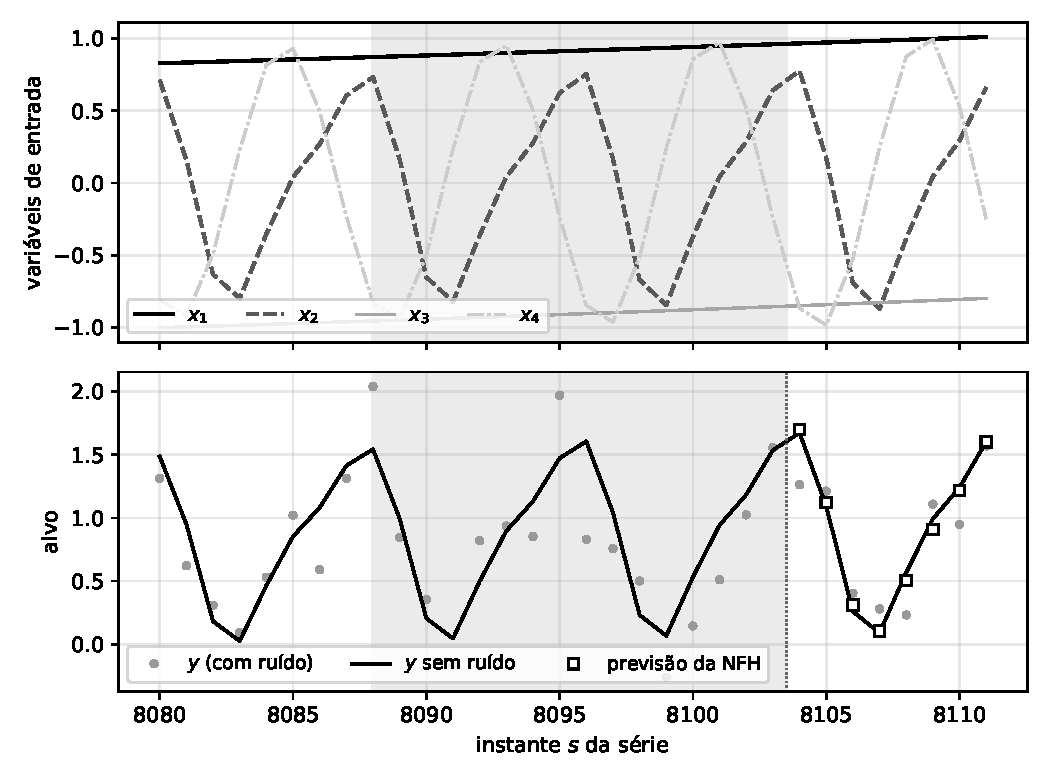
\includegraphics[width=0.85\textwidth]{figuras/fig_serie_janela.pdf}
\par\vspace{2pt}{\footnotesize Fonte: elaborado pelo autor.}
\end{figure}

O futuro real (com ruído) e o oráculo (sem ruído), em cada hora $j=0,\dots,7$, estão na Tabela~\ref{tab:fut}.

\begin{table}[H]
\centering
\caption{Futuro real e oráculo.}\label{tab:fut}
\footnotesize
\resizebox{\textwidth}{!}{%
\begin{tabular}{lrrrrrrrr}
\toprule
$j$ & 0 & 1 & 2 & 3 & 4 & 5 & 6 & 7 \\
\midrule
$y_j$ (real) & $1,262$ & $1,211$ & $0,4031$ & $0,2802$ & $0,2315$ & $1,109$ & $0,9487$ & $1,568$ \\
oráculo $x_1+x_2$ & $1,672$ & $1,092$ & $0,2590$ & $0,08994$ & $0,5683$ & $0,9916$ & $1,240$ & $1,602$ \\
\bottomrule
\end{tabular}
}
\par\vspace{2pt}{\footnotesize Fonte: elaborado pelo autor.}
\end{table}

\section{Passo 1: o backbone calcula $\bh$}\label{sec:h}

Cada um dos $16$ neurônios de $\bh$ faz o mesmo: multiplica cada um dos $64$ números de $\mathrm{vec}(\bX)$ por um peso, soma tudo, soma um viés e aplica $\tanh$, que comprime o resultado para $(-1,1)$. Mostramos as contas completas do neurônio $1$ (o primeiro; fixado antes de olhar): $h_1=\tanh\big(\sum_{k=1}^{64}W_{\Phi,1k}\,x_k+b_{\Phi,1}\big)$. A Tabela~\ref{tab:neuronio} lista, para cada posição $\ell$ e variável, o peso $w$ e o produto $w\cdot x$ (o $x$ está na Tabela~\ref{tab:X}).

\begin{table}[H]
\centering
\caption{Os 64 produtos $w\cdot x$ do neurônio 1 (3 algarismos significativos).}\label{tab:neuronio}
\footnotesize
\begin{tabular}{rrrrrrrrr}
\toprule
$\ell$ & $w$ ($\!x_1$) & $w\,x$ ($\!x_1$) & $w$ ($\!x_2$) & $w\,x$ ($\!x_2$) & $w$ ($\!x_3$) & $w\,x$ ($\!x_3$) & $w$ ($\!x_4$) & $w\,x$ ($\!x_4$) \\
\midrule
1 & $-0,0858$ & $-0,0748$ & $-0,0509$ & $-0,0373$ & $-0,0655$ & $0,0625$ & $-0,0829$ & $0,0686$ \\
2 & $-0,129$ & $-0,113$ & $-0,0219$ & $-0,00359$ & $0,0299$ & $-0,0284$ & $0,0400$ & $-0,0376$ \\
3 & $-0,0103$ & $-0,00912$ & $0,0456$ & $-0,0297$ & $-0,00580$ & $0,00547$ & $-0,0594$ & $0,0298$ \\
4 & $0,0290$ & $0,0257$ & $0,0722$ & $-0,0593$ & $0,0315$ & $-0,0295$ & $0,190$ & $0,0448$ \\
5 & $-0,0558$ & $-0,0499$ & $0,0461$ & $-0,0167$ & $0,0119$ & $-0,0110$ & $0,110$ & $0,0924$ \\
6 & $0,00177$ & $0,00160$ & $-0,0849$ & $-0,00360$ & $-0,124$ & $0,114$ & $-0,0350$ & $-0,0333$ \\
7 & $-0,0904$ & $-0,0819$ & $-0,197$ & $-0,0545$ & $-0,110$ & $0,101$ & $-0,0664$ & $-0,0336$ \\
8 & $-0,0676$ & $-0,0616$ & $-0,0158$ & $-0,00985$ & $0,0607$ & $-0,0553$ & $0,0153$ & $-0,00363$ \\
9 & $0,134$ & $0,123$ & $-0,00641$ & $-0,00484$ & $0,0395$ & $-0,0357$ & $-0,180$ & $0,152$ \\
10 & $0,197$ & $0,182$ & $-0,0161$ & $-0,00271$ & $0,0923$ & $-0,0828$ & $-0,0393$ & $0,0378$ \\
11 & $0,200$ & $0,186$ & $0,180$ & $-0,121$ & $-0,0407$ & $0,0363$ & $-0,0830$ & $0,0426$ \\
12 & $0,139$ & $0,130$ & $0,0456$ & $-0,0386$ & $0,00490$ & $-0,00434$ & $0,131$ & $0,0314$ \\
13 & $0,0407$ & $0,0383$ & $0,0375$ & $-0,0140$ & $-0,112$ & $0,0982$ & $0,231$ & $0,198$ \\
14 & $0,0681$ & $0,0646$ & $0,0538$ & $0,00235$ & $-0,0482$ & $0,0420$ & $0,149$ & $0,145$ \\
15 & $0,174$ & $0,166$ & $-0,0667$ & $-0,0191$ & $0,0768$ & $-0,0663$ & $0,161$ & $0,0836$ \\
16 & $0,101$ & $0,0966$ & $-0,181$ & $-0,116$ & $-0,00380$ & $0,00326$ & $-0,0273$ & $0,00665$ \\
\bottomrule
\end{tabular}
\par\vspace{2pt}{\footnotesize Fonte: elaborado pelo autor.}
\end{table}

Somando os 64 produtos: $0,6235$ (para $x_1$), $-0,5284$ ($x_2$), $0,1494$ ($x_3$) e $0,8243$ ($x_4$), total $\sum w\,x=1,069$. Somando o viés $b_{\Phi,1}=-0,4570$ obtém-se a pré-ativação $z=0,6118$, e então
\[h_1=\tanh(0,6118)=0,5454.\]
Os outros 15 neurônios seguem a mesma conta com seus próprios pesos. O vetor completo é, na Tabela~\ref{tab:h}, $\bh\in(-1,1)^{16}$ (diferença máxima de $8,9\times 10^{-8}$ contra o modelo em ponto flutuante de 32 bits).

\begin{table}[H]
\centering
\caption{A representação latente $\bh$.}\label{tab:h}
\scriptsize
\resizebox{\textwidth}{!}{%
\begin{tabular}{lrrrrrrrrrrrrrrrr}
\toprule
neurônio & 1 & 2 & 3 & 4 & 5 & 6 & 7 & 8 & 9 & 10 & 11 & 12 & 13 & 14 & 15 & 16 \\
\midrule
$h$ & $0,545$ & $0,232$ & $0,179$ & $-0,349$ & $0,499$ & $0,531$ & $0,348$ & $-0,0380$ & $0,162$ & $0,0951$ & $-0,0708$ & $-0,403$ & $0,308$ & $0,164$ & $-0,0978$ & $-0,396$ \\
\bottomrule
\end{tabular}
}
\par\vspace{2pt}{\footnotesize Fonte: elaborado pelo autor.}
\end{table}

\section{Passo 2: a cabeça calcula $\bc'=\bW\bh+\bb$}\label{sec:cprime}

\textbf{Aviso de índices:} daqui em diante, as linhas de $\bW$, as coordenadas de $\bc'$, $\bc$ e $\bD$ e as horas $j$ do horizonte começam em 0, enquanto os neurônios $k$ e as posições $\ell$ da janela começam em 1. Para conferir à mão, basta refazer a linha $i=0$; as outras seguem a mesma conta. A cabeça é uma camada linear: cada uma das $8$ linhas de $\bW$ faz o produto escalar com $\bh$ e soma o viés. As Tabelas~\ref{tab:W0} e~\ref{tab:W1} mostram $\bW$ e $\bb$; as Tabelas~\ref{tab:prod0} e~\ref{tab:prod1} mostram os produtos $W_{ik}h_k$ de todas as linhas, a soma de cada uma, o viés $b_i$ e o resultado $c'_i$.

\begin{table}[H]
\centering
\caption{A matriz $\bW\in\R^{8\times16}$, colunas 1 a 8 (3 algarismos significativos).}\label{tab:W0}
\footnotesize
\begin{tabular}{rrrrrrrrr}
\toprule
$i$ & 1 & 2 & 3 & 4 & 5 & 6 & 7 & 8 \\
\midrule
0 & $1,06$ & $1,05$ & $-0,102$ & $-0,486$ & $-0,595$ & $0,655$ & $0,292$ & $-0,691$ \\
1 & $-0,0460$ & $-0,838$ & $-0,539$ & $-0,199$ & $0,609$ & $0,235$ & $0,415$ & $-8,09\times 10^{-4}$ \\
2 & $-0,326$ & $0,459$ & $0,875$ & $-0,639$ & $1,03$ & $-0,458$ & $0,712$ & $-0,269$ \\
3 & $0,200$ & $0,309$ & $0,396$ & $-0,0291$ & $-0,733$ & $-0,0978$ & $-0,510$ & $0,0839$ \\
4 & $-0,0819$ & $0,361$ & $-0,909$ & $-0,185$ & $-0,00266$ & $-0,119$ & $-0,511$ & $0,387$ \\
5 & $-0,190$ & $0,287$ & $-0,145$ & $0,419$ & $0,0477$ & $0,384$ & $0,742$ & $-0,120$ \\
6 & $-0,0152$ & $0,119$ & $0,0238$ & $-0,0813$ & $0,0891$ & $0,0620$ & $-0,105$ & $-0,0255$ \\
7 & $-0,00302$ & $-0,0217$ & $-0,0437$ & $0,180$ & $-0,0510$ & $-0,0280$ & $0,131$ & $0,0111$ \\
\bottomrule
\end{tabular}
\par\vspace{2pt}{\footnotesize Fonte: elaborado pelo autor.}
\end{table}

\begin{table}[H]
\centering
\caption{A matriz $\bW\in\R^{8\times16}$, colunas 9 a 16 e viés $\bb$ (3 algarismos significativos).}\label{tab:W1}
\footnotesize
\begin{tabular}{rrrrrrrrrr}
\toprule
$i$ & 9 & 10 & 11 & 12 & 13 & 14 & 15 & 16 & $b_i$ \\
\midrule
0 & $-0,824$ & $-1,15$ & $0,522$ & $-0,987$ & $0,633$ & $-0,644$ & $-1,74$ & $-1,21$ & $0,393$ \\
1 & $1,51$ & $1,03$ & $0,430$ & $1,12$ & $-0,657$ & $0,0171$ & $-0,299$ & $-0,351$ & $0,126$ \\
2 & $-0,519$ & $0,445$ & $0,106$ & $-0,634$ & $0,578$ & $0,419$ & $-0,118$ & $0,0197$ & $-0,146$ \\
3 & $-1,08$ & $-0,0350$ & $-0,0102$ & $-0,00788$ & $0,190$ & $-0,338$ & $0,208$ & $0,327$ & $0,0618$ \\
4 & $0,833$ & $0,00263$ & $-0,177$ & $-0,842$ & $0,616$ & $0,733$ & $-0,505$ & $0,451$ & $-0,0229$ \\
5 & $0,534$ & $-0,755$ & $-0,838$ & $0,971$ & $0,632$ & $-0,0384$ & $0,0870$ & $-0,294$ & $-0,101$ \\
6 & $0,127$ & $-0,0427$ & $-0,0955$ & $-0,0497$ & $-0,0964$ & $-0,179$ & $0,160$ & $-0,120$ & $-0,109$ \\
7 & $-0,0412$ & $0,0172$ & $-0,147$ & $-0,119$ & $-0,0403$ & $-0,132$ & $-0,0574$ & $-0,0768$ & $0,0184$ \\
\bottomrule
\end{tabular}
\par\vspace{2pt}{\footnotesize Fonte: elaborado pelo autor.}
\end{table}

\begin{table}[H]
\centering
\caption{Produtos $W_{ik}h_k$ para $k=1,\dots,8$ (3 algarismos significativos). A linha $i=0$ define o nível da tendência e a linha $i=1$, sua inclinação.}\label{tab:prod0}
\footnotesize
\begin{tabular}{rrrrrrrrr}
\toprule
$i$ & 1 & 2 & 3 & 4 & 5 & 6 & 7 & 8 \\
\midrule
0 & $0,576$ & $0,244$ & $-0,0182$ & $0,169$ & $-0,297$ & $0,348$ & $0,102$ & $0,0262$ \\
1 & $-0,0251$ & $-0,194$ & $-0,0967$ & $0,0695$ & $0,304$ & $0,125$ & $0,144$ & $3,07\times 10^{-5}$ \\
2 & $-0,178$ & $0,106$ & $0,157$ & $0,223$ & $0,513$ & $-0,243$ & $0,248$ & $0,0102$ \\
3 & $0,109$ & $0,0716$ & $0,0710$ & $0,0102$ & $-0,366$ & $-0,0519$ & $-0,178$ & $-0,00318$ \\
4 & $-0,0447$ & $0,0837$ & $-0,163$ & $0,0646$ & $-0,00133$ & $-0,0633$ & $-0,178$ & $-0,0147$ \\
5 & $-0,104$ & $0,0666$ & $-0,0260$ & $-0,146$ & $0,0238$ & $0,204$ & $0,259$ & $0,00454$ \\
6 & $-0,00828$ & $0,0277$ & $0,00427$ & $0,0284$ & $0,0445$ & $0,0330$ & $-0,0367$ & $9,68\times 10^{-4}$ \\
7 & $-0,00165$ & $-0,00503$ & $-0,00784$ & $-0,0628$ & $-0,0254$ & $-0,0149$ & $0,0458$ & $-4,23\times 10^{-4}$ \\
\bottomrule
\end{tabular}
\par\vspace{2pt}{\footnotesize Fonte: elaborado pelo autor.}
\end{table}

\begin{table}[H]
\centering
\caption{Produtos $W_{ik}h_k$ para $k=9,\dots,16$, soma sobre todos os $k$, viés e $c'_i$ (3 algarismos significativos). A linha $i=0$ define o nível da tendência e a linha $i=1$, sua inclinação.}\label{tab:prod1}
\footnotesize
\resizebox{\textwidth}{!}{%
\begin{tabular}{rrrrrrrrrrrr}
\toprule
$i$ & 9 & 10 & 11 & 12 & 13 & 14 & 15 & 16 & $\sum_k$ & $b_i$ & $c'_i$ \\
\midrule
0 & $-0,133$ & $-0,109$ & $-0,0369$ & $0,398$ & $0,195$ & $-0,105$ & $0,170$ & $0,481$ & $2,010$ & $0,3931$ & $2,403$ \\
1 & $0,244$ & $0,0977$ & $-0,0305$ & $-0,452$ & $-0,202$ & $0,00280$ & $0,0293$ & $0,139$ & $0,1547$ & $0,1264$ & $0,2811$ \\
2 & $-0,0838$ & $0,0424$ & $-0,00752$ & $0,256$ & $0,178$ & $0,0685$ & $0,0115$ & $-0,00780$ & $1,294$ & $-0,1464$ & $1,147$ \\
3 & $-0,174$ & $-0,00333$ & $7,23\times 10^{-4}$ & $0,00318$ & $0,0585$ & $-0,0552$ & $-0,0204$ & $-0,130$ & $-0,6570$ & $0,06175$ & $-0,5952$ \\
4 & $0,135$ & $2,50\times 10^{-4}$ & $0,0125$ & $0,340$ & $0,189$ & $0,120$ & $0,0494$ & $-0,179$ & $0,3506$ & $-0,02287$ & $0,3277$ \\
5 & $0,0863$ & $-0,0718$ & $0,0594$ & $-0,392$ & $0,194$ & $-0,00628$ & $-0,00851$ & $0,117$ & $0,2601$ & $-0,1008$ & $0,1593$ \\
6 & $0,0206$ & $-0,00406$ & $0,00676$ & $0,0201$ & $-0,0297$ & $-0,0293$ & $-0,0156$ & $0,0474$ & $0,1099$ & $-0,1086$ & $0,001242$ \\
7 & $-0,00665$ & $0,00163$ & $0,0104$ & $0,0480$ & $-0,0124$ & $-0,0216$ & $0,00562$ & $0,0305$ & $-0,01688$ & $0,01837$ & $0,001491$ \\
\bottomrule
\end{tabular}
}
\par\vspace{2pt}{\footnotesize Fonte: elaborado pelo autor.}
\end{table}

Por escrito, para as duas primeiras linhas (as reticências escondem termos que estão nas Tabelas~\ref{tab:prod0} e~\ref{tab:prod1}):
\begin{align*}
c'_{0} &= \sum_{k=1}^{16}W_{0,k}h_k+b_0 = (1,06)(0,545) + (1,05)(0,232) + \cdots + (-1,21)(-0,396) + 0,3931\\
&= 2,010 + (0,3931) = 2,403\\[4pt]
c'_{1} &= \sum_{k=1}^{16}W_{1,k}h_k+b_1 = (-0,0460)(0,545) + (-0,838)(0,232) + \cdots + (-0,351)(-0,396) + 0,1264\\
&= 0,1547 + (0,1264) = 0,2811
\end{align*}
O vetor completo é $\bc'=(2,403;\allowbreak\ 0,2811;\allowbreak\ 1,147;\allowbreak\ -0,5952;\allowbreak\ 0,3277;\allowbreak\ 0,1593;\allowbreak\ 0,001242;\allowbreak\ 0,001491)$.

\subsection*{Normalização e divisão}
Multiplicando termo a termo por $\bD=\mathrm{diag}(0,3536;\allowbreak\ 0,6761;\allowbreak\ 0,5257;\allowbreak\ 0,7496;\allowbreak\ 0,5257;\allowbreak\ 0,5257;\allowbreak\ 1,000;\allowbreak\ 1,000)$ obtém-se $\bc=\bD\bc'=(0,8496;\allowbreak\ 0,1901;\allowbreak\ 0,6032;\allowbreak\ -0,4462;\allowbreak\ 0,1722;\allowbreak\ 0,08373;\allowbreak\ 0,001242;\allowbreak\ 0,001491)$. Os $q+1=2$ primeiros números são $\thT$, os $2K=4$ seguintes são $\thS=(a_1,b_1,a_2,b_2)$ e os $H-m=2$ últimos são $\bu$:
\begin{align*}
\thT&=(0,8496;\allowbreak\ 0,1901) &&\text{(nível $\theta_{T,0}$ e inclinação $\theta_{T,1}$)}\\
\thS&=(0,6032;\allowbreak\ -0,4462;\allowbreak\ 0,1722;\allowbreak\ 0,08373) &&\text{(cosseno e seno dos harmônicos 1 e 2)}\\
\bu&=(0,001242;\allowbreak\ 0,001491) &&\text{(coeficientes do resíduo)}
\end{align*}

\section{Passo 3: sintetizar $\bT$, $\bS$, $\bR$ e conferir a soma}\label{sec:TSR}

Agora cada componente sai de um produto simples: $\bT=\bP^\top\thT$, $\bS=\bFt^\top\thS$, $\bR=\bQ\bu$ e $\byh=\bT+\bS+\bR$. Exemplo na hora $j=4$ (fixada em $\lfloor H/2\rfloor$), com $\tau=0,500$:
\begin{align*}
T_{4}&=\theta_{T,0}\cdot 1+\theta_{T,1}\,\tau=(0,8496)(1)+(0,1901)(0,500)=0,9447,\\
S_{4}&=\sum_{i=1}^{4}\widetilde F_{i,4}\,\theta_{S,i}\\
&=(-0,952)(0,603) + (0,115)(-0,446) + (1,05)(0,172) + (0,0476)(0,0837)=-0,4413,\\
R_{4}&=\sum_{i=1}^{2}Q_{4,i}\,u_i=(0,381)(0,00124)+(0,439)(0,00149)=0,001127,\\
\hat y_{4}&=T_{4}+S_{4}+R_{4}=0,9447+(-0,4413)+(0,001127)=0,5045.
\end{align*}
A Tabela~\ref{tab:TSR} repete a conta para as $8$ horas. O maior erro de $T+S+R$ contra $\byh$ calculado por $\bM\bc$ é $5,6\times 10^{-17}$, a soma é exata a menos do arredondamento.

\begin{table}[H]
\centering
\caption{Decomposição da previsão da NFH hora a hora.}\label{tab:TSR}
\small
\begin{tabular}{rrrrrrrr}
\toprule
$j$ & $T_j$ & $S_j$ & $R_j$ & $T_j+S_j+R_j$ & $\hat y_j$ & oráculo & real \\
\midrule
0 & $0,8496$ & $0,8481$ & $-3,537\times 10^{-5}$ & $1,698$ & $1,698$ & $1,672$ & $1,262$ \\
1 & $0,8734$ & $0,2467$ & $-7,451\times 10^{-5}$ & $1,120$ & $1,120$ & $1,092$ & $1,211$ \\
2 & $0,8971$ & $-0,5873$ & $4,605\times 10^{-4}$ & $0,3103$ & $0,3103$ & $0,2590$ & $0,4031$ \\
3 & $0,9209$ & $-0,8154$ & $-8,965\times 10^{-4}$ & $0,1046$ & $0,1046$ & $0,08994$ & $0,2802$ \\
4 & $0,9447$ & $-0,4413$ & $0,001127$ & $0,5045$ & $0,5045$ & $0,5683$ & $0,2315$ \\
5 & $0,9684$ & $-0,05842$ & $-0,001017$ & $0,9090$ & $0,9090$ & $0,9916$ & $1,109$ \\
6 & $0,9922$ & $0,2220$ & $6,313\times 10^{-4}$ & $1,215$ & $1,215$ & $1,240$ & $0,9487$ \\
7 & $1,016$ & $0,5856$ & $-1,953\times 10^{-4}$ & $1,601$ & $1,601$ & $1,602$ & $1,568$ \\
\bottomrule
\end{tabular}
\par\vspace{2pt}{\footnotesize Fonte: elaborado pelo autor.}
\end{table}

\textbf{A média de $\bT$ é a média da previsão.} Como $\bFt\perp\bP$ e $\bQ\perp\bP$ e a primeira linha de $\bP$ é toda de uns, $\bS$ e $\bR$ têm média zero. Numericamente: média de $\bT$ = $0,9328$ e média de $\byh$ = $0,9328$. Por isso o nível médio previsto fica todo em $\bT$ e o ciclo não tem como ``roubar'' nível.

\section{Passo 4: balanço de energia e harmônicos}\label{sec:energia}

Como $\bT$ (sem a média), $\bS$ e $\bR$ são ortogonais, a energia da previsão centrada, $\En=\|\byh-\bar y\|^2$ (não confundir com as $E$ épocas extras da Seção~\ref{sec:selecao}), se reparte sem sobras: $\varepsilon_T=\|\bT-\bar y\|^2/\En$, $\varepsilon_S=\|\bS\|^2/\En$, $\varepsilon_R=\|\bR\|^2/\En$, com $\varepsilon_T+\varepsilon_S+\varepsilon_R=1$. Aqui $\bar y=0,9328$ (a média dos $H$ valores previstos) e $\En=2,404$. Resulta $\varepsilon_T=0,986\,\%$, $\varepsilon_S=99,0\,\%$ e $\varepsilon_R=1,57\times 10^{-4}\,\%$ (soma $1,0000000$). Ou seja, na previsão centrada, a quase totalidade da variação é sazonal, e o resíduo é desprezível: a previsão já \emph{nasce} dentro do espaço estrutural. Esta é uma janela só; que isso se deva à penalização $\lambda$ não sai daqui, e a comparação que a sustenta, feita na validação com 5 sementes, está na Seção~\ref{sec:selecao} (com $p=16$ e $n=1000$, RMSE de validação $0,3342$ sem penalização e $0,3148$ com $\lambda=1000$, menor em 5 das 5 sementes).

Cada harmônico $k$ tem coeficientes $(a_k,b_k)$ do cosseno e do seno; $a_k\cos(2\pi k\tau)+b_k\sen(2\pi k\tau)=A_k\cos(2\pi k\tau-\varphi_k)$ com amplitude $A_k=\sqrt{a_k^2+b_k^2}$ e fase $\varphi_k=\operatorname{atan2}(b_k,a_k)$. A participação $e_k=\langle \bS_k,\bS\rangle/\En$ ($\bS_k$ é a parte de $\bS$ do harmônico $k$) é a fatia da energia que o harmônico $k$ carrega. Na Tabela~\ref{tab:harm}, as colunas da NFH e da verdade (Seção~\ref{sec:verdade}) permitem comparar.

\begin{table}[H]
\centering
\caption{Harmônicos da NFH e da verdade (oráculo) nesta janela.}\label{tab:harm}
\footnotesize
\begin{tabular}{rrrrrrrrrr}
\toprule
$k$ & período & $a_k$ & $b_k$ & $A_k$ & $\varphi_k$ (rad) & $e_k$ & $A_k$ verdade & $\varphi_k$ verdade & $e_k$ verdade \\
\midrule
1 & $8,00$ & $0,6032$ & $-0,4462$ & $0,7503$ & $-0,6369$ & $92,0\,\%$ & $0,7404$ & $-0,6915$ & $88,4\,\%$ \\
2 & $4,00$ & $0,1722$ & $0,08373$ & $0,1915$ & $0,4525$ & $6,99\,\%$ & $0,2224$ & $0,5038$ & $9,47\,\%$ \\
\bottomrule
\end{tabular}
\par\vspace{2pt}{\footnotesize Fonte: elaborado pelo autor.}
\end{table}

\section{A verdade: a mesma decomposição aplicada ao oráculo}\label{sec:verdade}

Podemos decompor qualquer vetor de $\R^H$ pelas mesmas bases, sem rede nenhuma: $\thT=(\bP\bP^\top)^{-1}\bP\mathbf y$, $\thS=(\bFt\bFt^\top)^{-1}\bFt\mathbf y$, $\bu=\bQ^\top\mathbf y$ (as ``fórmulas de identificabilidade'': dada a previsão, os coeficientes são únicos). Aplicadas ao oráculo $\mathbf y^\star=x_1+x_2$ (Tabela~\ref{tab:fut}) dão $\thT^\star=(0,8176;\allowbreak\ 0,2783)$, $\thS^\star=(0,5704;\allowbreak\ -0,4721;\allowbreak\ 0,1947;\allowbreak\ 0,1073)$ e $\bu^\star=(-7,733\times 10^{-4};\allowbreak\ 4,987\times 10^{-4})$; o asterisco marca, daqui em diante, a mesma grandeza calculada sobre o oráculo (a ``verdade'') em vez da previsão da NFH. A energia da verdade se reparte em $\varepsilon_T^\star=2,11\,\%$, $\varepsilon_S^\star=97,9\,\%$ e $\varepsilon_R^\star=3,51\times 10^{-5}\,\%$, definidos como $\varepsilon_T,\varepsilon_S,\varepsilon_R$ do Passo 4, com $\mathbf y^\star$ no lugar de $\byh$.

\paragraph{De onde deveriam vir esses números.} No horizonte, $x_2(s_0+j)=A_s[\cos(2\pi j/8+\psi_1)+0{,}3\cos(2\pi j/4+\psi_2)]$ com $\psi_1=2\pi s_0/8+0,7000\equiv0,7000$ e $\psi_2=2\pi s_0/4-0,5000\equiv5,783$ (módulo $2\pi$; aqui $s_0=8096$). Com a amplitude trocada pela média no horizonte, $\bar A=0,7432$, e $\cos(\omega j+\psi)=\cos\psi\cos\omega j-\sen\psi\sen\omega j$, os coeficientes esperados do seno e do cosseno são $\beta=\bar A(\cos\psi_1,\,-\sen\psi_1,\,0{,}3\cos\psi_2,\,-0{,}3\sen\psi_2)=(0,5684;\allowbreak\ -0,4788;\allowbreak\ 0,1957;\allowbreak\ 0,1069)$, que se comparam a $\thS^\star=(0,5704;\allowbreak\ -0,4721;\allowbreak\ 0,1947;\allowbreak\ 0,1073)$ (diferem porque $A_s$ varia no horizonte). Já a reta de $x_1$ no horizonte é $\boldsymbol\alpha_{x_1}=(0,9176;\allowbreak\ 0,04844)$ (nível e inclinação em $\tau$). Os ciclos trazem uma reta embutida, $\boldsymbol\alpha\boldsymbol\beta=(-0,08914;\allowbreak\ 0,2038)$, que o desenho de $\bFt$ tirou da sazonalidade e devolveu à tendência: $\thT^\star\approx\boldsymbol\alpha_{x_1}+\boldsymbol\alpha\boldsymbol\beta=(0,8227;\allowbreak\ 0,2655)$, contra $\thT^\star=(0,8176;\allowbreak\ 0,2783)$ calculado diretamente.

\paragraph{Erro da NFH contra a verdade.} Na Figura~\ref{fig:TSR} aparecem os componentes; a diferença dos coeficientes é $\thT-\thT^\star=(0,03202;\allowbreak\ -0,08828)$ e $\thS-\thS^\star=(0,03281;\allowbreak\ 0,02595;\allowbreak\ -0,02248;\allowbreak\ -0,02360)$. Em unidade de previsão, o erro máximo é $0,08262$, o RMSE da NFH contra o oráculo nesta janela é $0,04442$ e contra o futuro real, $0,2303$. Por componente, o maior desvio absoluto é $0,04523$ em $\bT$, $0,05810$ em $\bS$ e $0,001363$ em $\bR$.

\begin{figure}[H]
\centering
\caption{Componentes da NFH (quadrados pretos, linha contínua) e da verdade (círculos cinza médio, linha tracejada) em cada hora do horizonte: tendência $T$, sazonalidade $S$ e resíduo $R$.}\label{fig:TSR}
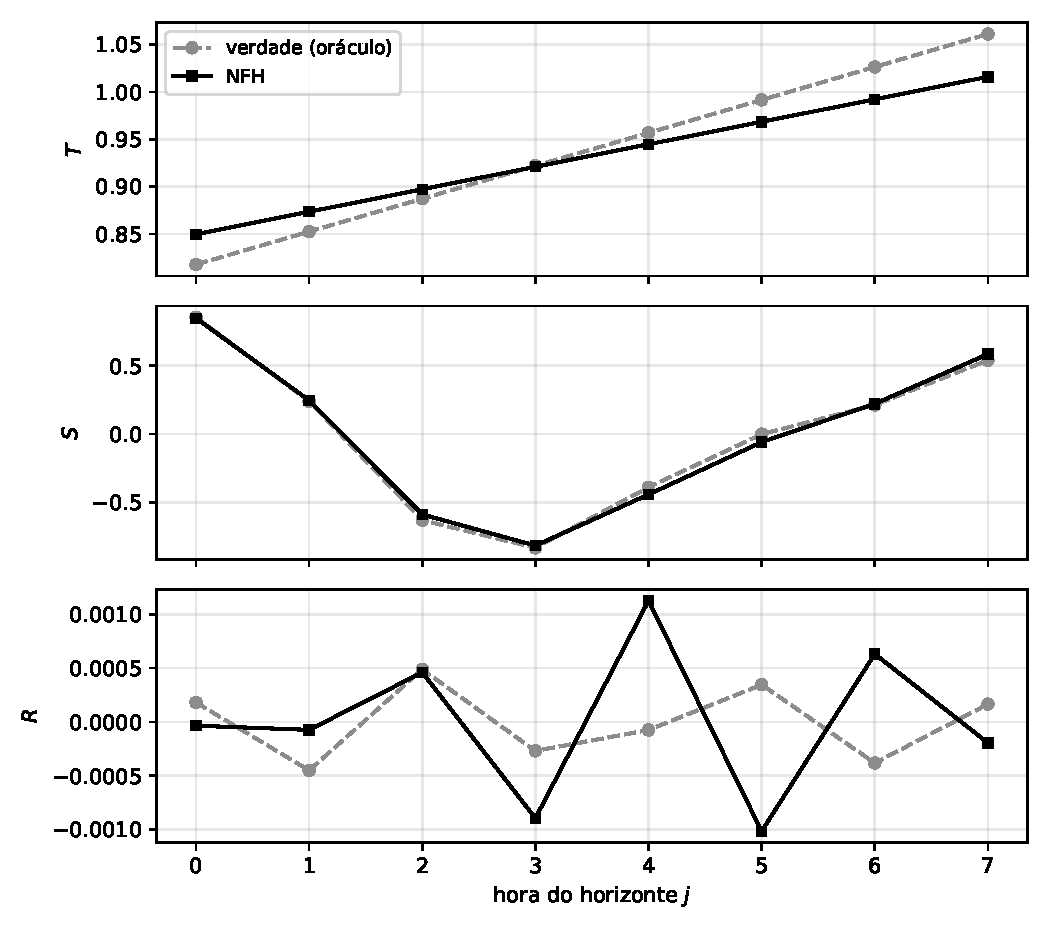
\includegraphics[width=0.85\textwidth]{figuras/fig_TSR.pdf}
\par\vspace{2pt}{\footnotesize Fonte: elaborado pelo autor.}
\end{figure}

\section{A camada densa da mesma semente: só dá para decompor depois}\label{sec:densa}

A densa da semente 10 usa o mesmo backbone treinado do mesmo jeito, mas sua cabeça escreve $\hat{\mathbf y}$ direto. Para explicá-la é preciso decompor a previsão depois, pelas mesmas fórmulas de identificabilidade. A previsão da densa nesta janela é $(1,840;\allowbreak\ 1,069;\allowbreak\ 0,2029;\allowbreak\ 0,1124;\allowbreak\ 0,5892;\allowbreak\ 0,9879;\allowbreak\ 1,377;\allowbreak\ 1,695)$. Decomposta: $\thT=(0,8444;\allowbreak\ 0,3197)$, $\thS=(0,5780;\allowbreak\ -0,6287;\allowbreak\ 0,1835;\allowbreak\ 0,03340)$, $\bu=(0,03939;\allowbreak\ -0,002448)$. As participações de energia são $\varepsilon_T=2,29\,\%$, $\varepsilon_S=97,7\,\%$, $\varepsilon_R=0,0532\,\%$. O resíduo da densa carrega $0,0532\,\%$ da energia centrada, contra $1,57\times 10^{-4}\,\%$ na NFH. Isso é compatível com o efeito de penalizar o resíduo, mas uma janela e uma semente não o demonstram; o que a seleção traz sobre a penalização está na Seção~\ref{sec:selecao} (com $p=16$ e $n=1000$, RMSE de validação $0,3342$ sem penalização e $0,3148$ com $\lambda=1000$, menor em 5 das 5 sementes). O RMSE contra o oráculo nesta janela é $0,08692$ (densa) e $0,04442$ (NFH); contra o futuro real, $0,3093$ e $0,2303$. Uma janela só ilustra; as duas são comparadas no teste inteiro na Seção~\ref{sec:resumo}.

\section{Conversão entre a NFH e a camada densa}\label{sec:conv}

A NFH não é um modelo diferente da densa: é a mesma família linear com os coeficientes reorganizados. Como $\byh=\bM\bD(\bW\bh+\bb)$, uma camada densa equivalente tem $\bW'=\bM\bD\bW$ e $\bb'=\bM\bD\bb$. Por exemplo, o elemento $W'_{0,0}=\sum_i(\bM\bD)_{0,i}W_{i,0}$ é a soma de 8 produtos, e a densa equivalente produz, para esta janela, a mesma previsão da NFH com diferença máxima $2,2\times 10^{-16}$. A volta é $\bW=(\bM\bD)^{-1}\bW'$ e $\bb=(\bM\bD)^{-1}\bb'$; como $\bM\bD$ é inversível (condição $4,209$), $\bW$ e $\bb$ voltam com erro máximo $4,4\times 10^{-16}$ e $1,1\times 10^{-16}$. A primeira linha da densa equivalente é $\bW'_{0,:}=(0,145;\allowbreak\ 0,402;\allowbreak\ -0,270;\allowbreak\ -0,483;\allowbreak\ 0,563;\allowbreak\ 0,00775;\allowbreak\ 0,382;\allowbreak\ -0,227;\allowbreak\ 0,349;\allowbreak\ -0,0869;\allowbreak\ 0,312;\allowbreak\ -1,04;\allowbreak\ 0,428;\allowbreak\ 0,401;\allowbreak\ -1,01;\allowbreak\ -0,399)$ (16 números) e $b'_0=0,07970$. Na direção densa $\to$ NFH, aplicada à densa treinada da semente 10, a NFH obtida prevê o mesmo que a densa em todo o teste, com diferença máxima $1,2\times 10^{-6}$ (precisão de 32 bits). Isso é o que permite, em outros experimentos, converter uma rede já treinada e só depois ajustá-la.

\section{A ambiguidade do N-BEATS-I na mesma previsão}\label{sec:nbeats}

O N-BEATS interpretável também divide a previsão em tendência e sazonalidade, mas com blocos que somam bases \emph{sem exigir ortogonalidade}. Para ver o problema, usa-se para a tendência um polinômio de grau 2 ($3$ colunas) e para a sazonalidade uma constante mais os harmônicos 1 a 3 ($7$ colunas). As duas bases juntas têm posto $8$ em $\R^{8}$, então há mais colunas que dimensões, e a mesma previsão $\byh$ admite infinitas divisões. A Tabela~\ref{tab:nb} mostra duas, ambas com erro de soma de no máximo $8,9\times 10^{-16}$: a divisão (a) é a de menor norma; a (b) passa uma constante $+1$ da sazonalidade para a tendência. A média da sazonalidade vai de $0,4642$ em (a) para $-0,5358$ em (b), e a tendência de $0,4686$ para $1,469$: o ``nível'' depende de uma escolha arbitrária. Na NFH a divisão é única, e a tendência vale $0,9328$ em média, igual à média da previsão (Seção~\ref{sec:TSR}).

\begin{table}[H]
\centering
\caption{Duas divisões da mesma previsão no estilo N-BEATS-I (a primeira e a segunda) e a divisão única da NFH.}\label{tab:nb}
\footnotesize
\begin{tabular}{rrrrrrrr}
\toprule
$j$ & $T$ (a) & $S$ (a) & $T$ (b) & $S$ (b) & $T$ NFH & $S+R$ NFH & $\hat y_j$ \\
\midrule
0 & $0,4642$ & $1,234$ & $1,464$ & $0,2335$ & $0,8496$ & $0,8481$ & $1,698$ \\
1 & $0,4642$ & $0,6558$ & $1,464$ & $-0,3442$ & $0,8734$ & $0,2466$ & $1,120$ \\
2 & $0,4648$ & $-0,1545$ & $1,465$ & $-1,155$ & $0,8971$ & $-0,5868$ & $0,3103$ \\
3 & $0,4661$ & $-0,3615$ & $1,466$ & $-1,361$ & $0,9209$ & $-0,8163$ & $0,1046$ \\
4 & $0,4680$ & $0,03648$ & $1,468$ & $-0,9635$ & $0,9447$ & $-0,4402$ & $0,5045$ \\
5 & $0,4705$ & $0,4385$ & $1,471$ & $-0,5615$ & $0,9684$ & $-0,05943$ & $0,9090$ \\
6 & $0,4737$ & $0,7412$ & $1,474$ & $-0,2588$ & $0,9922$ & $0,2227$ & $1,215$ \\
7 & $0,4775$ & $1,124$ & $1,477$ & $0,1239$ & $1,016$ & $0,5854$ & $1,601$ \\
\bottomrule
\end{tabular}
\par\vspace{2pt}{\footnotesize Fonte: elaborado pelo autor.}
\end{table}

\section{Integrated Gradients por componente}\label{sec:ig}

Até aqui explicamos \emph{o que} a previsão contém. Falta dizer \emph{quais entradas} produzem cada parte. Para qualquer função escalar $g$ da janela, o Integrated Gradients (IG) com referência nula atribui à entrada $x_{\ell v}$ o valor $\mathrm{IG}_{\ell v}=x_{\ell v}\int_0^1\partial g/\partial x_{\ell v}(\alpha\bX)\,d\alpha$ e satisfaz a \emph{completude}: $\sum_{\ell v}\mathrm{IG}_{\ell v}=g(\bX)-g(\mathbf 0)$. A integral é calculada pela regra do ponto médio com 256 passos. Como a NFH expõe $\bT$ e $\bS$ como saídas, podemos aplicar o IG a um funcional de cada uma, em vez de a um número só: $g_T(\bX)=\overline{\bT}$ (o nível médio da tendência) e $g_S(\bX)=\|\bS\|^2$ (a energia sazonal). Somando as atribuições sobre as 16 linhas, obtém-se a contribuição de cada variável.

\paragraph{Verdade de referência.} Por construção, $x_1$ conduz a tendência e $x_2$ o ciclo. Para ter uma referência numérica e não só uma frase, aplica-se o mesmo IG à função do oráculo, $\mathbf y^\star(\bX)=x_1+x_2$ (últimas 8 linhas), com os mesmos $g_T$ e $g_S$ (a energia sazonal calculada pelo projetor sobre $\bFt$). Essa é a atribuição ``certa'' que um bom modelo deveria reproduzir. Os resultados estão na Tabela~\ref{tab:ig} e na Figura~\ref{fig:IG}.

\begin{table}[H]
\centering
\caption{IG por variável (somado sobre as linhas da janela). Participação é o valor absoluto da atribuição da variável dividido pela soma dos valores absolutos. Colunas ``verdade'': IG da função do oráculo.}\label{tab:ig}
\footnotesize
\resizebox{\textwidth}{!}{%
\begin{tabular}{lrrrrrrrr}
\toprule
variável & $g_T$ NFH & part. & $g_T$ verdade & part. & $g_S$ NFH & part. & $g_S$ verdade & part. \\
\midrule
$x_1$ & $1,025$ & $95,1\,\%$ & $0,9388$ & $99,9\,\%$ & $0,001481$ & $0,0521\,\%$ & $3,241\times 10^{-4}$ & $0,0137\,\%$ \\
$x_2$ & $-0,01728$ & $1,60\,\%$ & $5,593\times 10^{-4}$ & $0,0595\,\%$ & $2,609$ & $91,8\,\%$ & $2,363$ & $100,0\,\%$ \\
$x_3$ & $0,01079$ & $1,00\,\%$ & $0$ & $0\,\%$ & $-0,06000$ & $2,11\,\%$ & $0$ & $0\,\%$ \\
$x_4$ & $-0,02446$ & $2,27\,\%$ & $0$ & $0\,\%$ & $-0,1729$ & $6,08\,\%$ & $0$ & $0\,\%$ \\
soma & $0,9937$ &  & $0,9394$ &  & $2,377$ &  & $2,363$ &  \\
$g(\bX)-g(\mathbf 0)$ & $0,9937$ &  & $0,9394$ &  & $2,377$ &  & $2,363$ &  \\
erro de completude & $5,0\times 10^{-7}$ &  & $2,2\times 10^{-16}$ &  & $9,4\times 10^{-7}$ &  & $8,9\times 10^{-16}$ &  \\
\bottomrule
\end{tabular}
}
\par\vspace{2pt}{\footnotesize Fonte: elaborado pelo autor.}
\end{table}

Lendo a tabela: para a tendência, $x_1$ recebe $95,1\,\%$ da atribuição de $g_T$ na NFH, contra $99,9\,\%$ na verdade de referência; para o ciclo, $x_2$ recebe $91,8\,\%$ de $g_S$ na NFH, contra $100,0\,\%$ na referência. Os distratores $x_3$ e $x_4$ somam $3,27\,\%$ em $g_T$ e $8,19\,\%$ em $g_S$. A atribuição da NFH aponta as mesmas variáveis que a construção da série, e a pequena parte que vai para os distratores é erro de estimação do modelo (a referência dá a eles $0\,\%$ e $0\,\%$). A completude vale com erro de ordem $9,4\times 10^{-7}$ (a regra do ponto médio com 256 passos). Conferência extra: o IG do nível médio da previsão, $\overline{\byh}$, coincide com o de $g_T$ (diferença máxima entre as atribuições $2,8\times 10^{-17}$), como deve ser, pois $\overline{\bT}=\overline{\byh}$.

\begin{figure}[H]
\centering
\caption{Participação de cada variável nos funcionais $g_T$ (painel a) e $g_S$ (painel b): barras cinza escuro para a NFH e barras cinza claro com contorno para a verdade de referência (IG da função do oráculo).}\label{fig:IG}
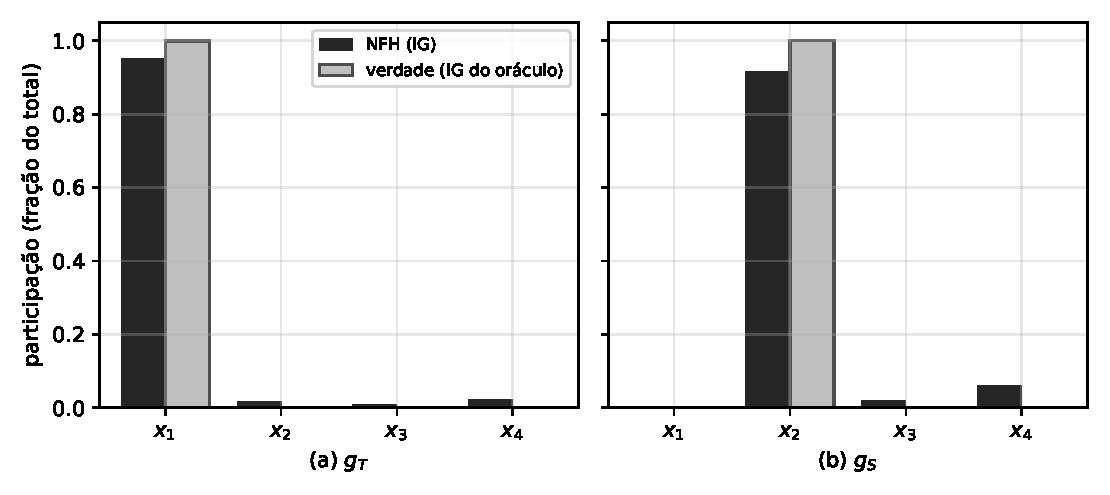
\includegraphics[width=0.9\textwidth]{figuras/fig_IG.pdf}
\par\vspace{2pt}{\footnotesize Fonte: elaborado pelo autor.}
\end{figure}

\section{Explicação abdutiva: quais neurônios sustentam a inclinação da tendência}\label{sec:abd}

Os IG mostram quais \emph{entradas} pesam, mas não dão garantia. Uma explicação \emph{abdutiva} procura um conjunto mínimo de características que, mantidas fixas, \emph{garantem} uma propriedade, quaisquer que sejam os valores das outras. Aqui as características são os $16$ neurônios de $\bh$, cada um em $[-1,1]$ (a imagem de $\tanh$). A propriedade é: ``a inclinação da tendência $\theta_{T,1}(\bh')=\sum_k w_k h'_k+w_0$ mantém o sinal e pelo menos metade do valor atual''. Como $\theta_{T,1}(\bh)=0,1901$ é positiva, escrevemos $s=1$ e exigimos $s\,\theta_{T,1}(\bh')\ge\xi=|\theta_{T,1}(\bh)|/2=0,09503$. Os pesos da inclinação são $w_k=s\,D_{11}W_{1,k}$ e $w_0=s\,D_{11}b_1$, com $D_{11}=0,6761$ (a coordenada de índice 1 de $\bD$; os índices de $\bc'$, $\bD$ e das linhas de $\bW$ começam em 0, como nas tabelas do Passo 2, enquanto os dos neurônios $k$ começam em 1).

\paragraph{Margens.} Se nenhum neurônio é fixado, o pior caso põe cada $h'_k=-\operatorname{sinal}(w_k)$ e vale $\Gamma_\emptyset=w_0-\sum_k|w_k|=-5,522$, abaixo de $\xi$. Fixar o neurônio $k$ no seu valor real $h_k$ melhora esse pior caso em $\delta_k=w_kh_k+|w_k|\ge0$ (o ganho). Para um conjunto $\mathcal A$ de neurônios fixados, o pior caso é $\Gamma(\mathcal A)=\Gamma_\emptyset+\sum_{k\in\mathcal A}\delta_k$, e $\mathcal A$ \emph{garante} a propriedade se $\Gamma(\mathcal A)\ge\xi$. Como os ganhos se somam, o menor conjunto que garante a propriedade vem de escolher os maiores ganhos primeiro (ordem gulosa). A Tabela~\ref{tab:gan} traz $w_k$, $h_k$, o ganho e a posição na ordem gulosa.

\begin{table}[H]
\centering
\caption{Ganhos $\delta_k=w_kh_k+|w_k|$ e posição na ordem gulosa.}\label{tab:gan}
\footnotesize
\begin{tabular}{rrrrr}
\toprule
$k$ & $w_k$ & $h_k$ & $\delta_k$ & posição \\
\midrule
1 & $-0,03109$ & $0,5454$ & $0,01414$ & 14 \\
2 & $-0,5663$ & $0,2319$ & $0,4350$ & 5 \\
3 & $-0,3646$ & $0,1793$ & $0,2993$ & 9 \\
4 & $-0,1346$ & $-0,3490$ & $0,1816$ & 13 \\
5 & $0,4120$ & $0,4993$ & $0,6176$ & 3 \\
6 & $0,1586$ & $0,5311$ & $0,2428$ & 11 \\
7 & $0,2803$ & $0,3485$ & $0,3780$ & 6 \\
8 & $-5,471\times 10^{-4}$ & $-0,03797$ & $5,679\times 10^{-4}$ & 16 \\
9 & $1,021$ & $0,1616$ & $1,186$ & 1 \\
10 & $0,6944$ & $0,09512$ & $0,7604$ & 2 \\
11 & $0,2908$ & $-0,07083$ & $0,2702$ & 10 \\
12 & $0,7579$ & $-0,4035$ & $0,4521$ & 4 \\
13 & $-0,4446$ & $0,3076$ & $0,3078$ & 8 \\
14 & $0,01156$ & $0,1636$ & $0,01345$ & 15 \\
15 & $-0,2022$ & $-0,09783$ & $0,2220$ & 12 \\
16 & $-0,2374$ & $-0,3965$ & $0,3315$ & 7 \\
\bottomrule
\end{tabular}
\par\vspace{2pt}{\footnotesize Fonte: elaborado pelo autor.}
\end{table}

Acumulando os ganhos nessa ordem (9, 10, 5, 12, 2, 7, 16, 13, 3, 11, 6, 15, 4, \ldots), o pior caso garantido passa de $-5,522$ para $-4,337$, $-3,576$, $\dots$ e cruza $\xi=0,09503$ com $k^*=13$ neurônios, em que $\Gamma=0,1619$. Com um neurônio a menos ($k^*-1=12$), $\Gamma=-0,01970<\xi$, então 13 é o mínimo. A explicação é o conjunto $\mathcal A^*=\{2, 3, 4, 5, 6, 7, 9, 10, 11, 12, 13, 15, 16\}$: se esses 13 neurônios forem mantidos nos valores atuais, a inclinação mantém o sinal e pelo menos metade do valor para \emph{qualquer} valor dos outros 3 neurônios em $[-1,1]$. Note o custo: $k^*=13$ de 16 neurônios é $81\,\%$ da camada, de modo que a explicação mínima fixa a maior parte dela; é uma garantia, não uma explicação curta. A Figura~\ref{fig:abd} mostra o acumulado.

\begin{figure}[H]
\centering
\caption{Pior valor garantido de $s\,\theta_{T,1}$ conforme se fixam neurônios, na ordem gulosa (pretos, linha contínua) e na ordem dos Integrated Gradients (cinza médio, tracejada). A linha pontilhada é $\xi$; a vertical cinza claro marca $k^*$ da ordem gulosa.}\label{fig:abd}
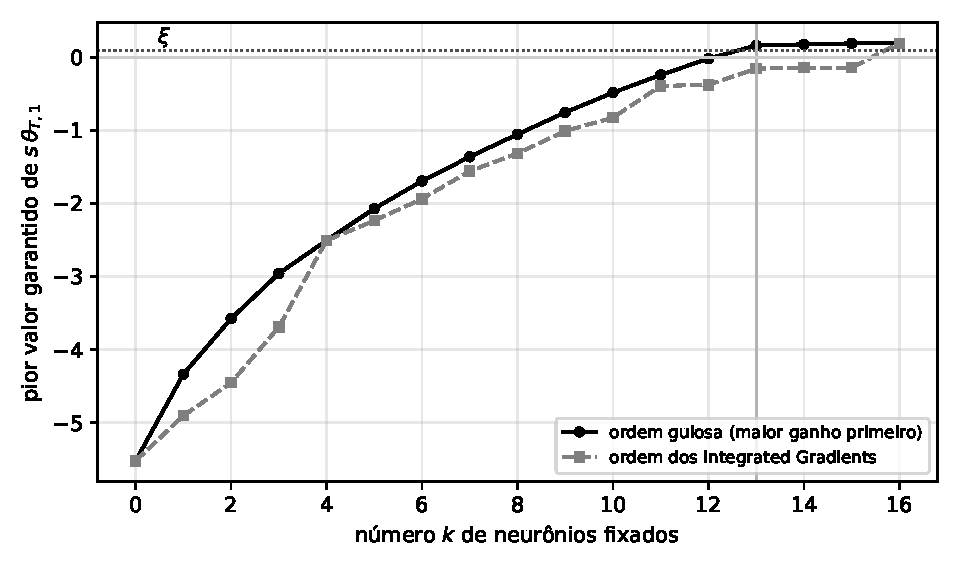
\includegraphics[width=0.75\textwidth]{figuras/fig_abdutiva.pdf}
\par\vspace{2pt}{\footnotesize Fonte: elaborado pelo autor.}
\end{figure}

\paragraph{Verificação por amostragem.} Para conferir sem confiar só na álgebra, sorteiam-se $10\,000$ vetores $\bh'$ uniformes em $[-1,1]^{16}$, com os neurônios de $\mathcal A^*$ fixados nos valores reais: o número de violações da propriedade é 0. Retirando o último neurônio incluído (o 4), a mesma amostragem encontra 2753 violações em $10\,000$, e o pior completamento (cada neurônio livre no extremo desfavorável) leva $s\,\theta_{T,1}$ a $-0,01970$, abaixo de $\xi$; calculando $\theta_{T,1}$ diretamente com os pesos da cabeça nesse $\bh'$ obtém-se $-0,01970$, o mesmo valor. A amostragem não prova nada (só a conta das margens prova), mas confirma que a conta e o código concordam.

\paragraph{Comparação com a ordem dos Integrated Gradients.} Foi testada uma única alternativa à ordem gulosa: fixar os neurônios em ordem decrescente de $|w_k(h_k-\bar h_k)|$, com $\bar h_k$ a média de $h_k$ nas janelas de treino. É uma atribuição ``estilo IG'' (linear, relativa à média), não o Integrated Gradients da seção anterior. A ordem obtida é 5, 12, 10, 9, 11, 3, \ldots e o limiar $\xi$ só é atingido com $k_{\mathrm{IG}}=16$ neurônios, contra $k^*=13$ da ordem gulosa. Neste exemplo, essa ordem precisou de mais neurônios que o mínimo. Isso mostra que, aqui, o que pesa na média não coincide com o que sustenta a garantia; é um caso, e outra ordem ou outra janela podem dar outro resultado.

\paragraph{Limites da garantia.} A garantia vale na última camada (sobre $\bh$ como se fosse livre em $[-1,1]^p$, sem passar pelo backbone) e é relativa à caixa $[-1,1]^p$. Ela não diz quais entradas de $\bX$ geram esses neurônios.

\section{De uma janela para o teste inteiro}\label{sec:resumo}

Uma janela só ilustra. A Tabela~\ref{tab:conf} traz o teste inteiro, em cada semente da confirmação, com as duas últimas colunas do controle adicional descrito a seguir. Nela, a semente 10 é a explicada neste documento. As médias e os desvios estão na primeira página.

\paragraph{Controle adicional: a densa projetada em $\bT\oplus\bS$.} Depois da confirmação, e a pedido de uma auditoria externa, calculou-se com o código do projeto (o projetor $\bQ\bQ^\top$ de \texttt{exemplo\_livro/treinar.py}) o que acontece se a previsão da camada densa for projetada em $\bT\oplus\bS$ \emph{sem treino}: $\byh_{\mathrm{proj}}=\byh-\bQ\bQ^\top\byh$, isto é, a decomposição pura com o resíduo descartado. Para cada semente 10 a 19 retreinou-se a densa (a mesma do critério; o RMSE e o MAE reproduzem os de \texttt{confirmacao.csv} com diferença máxima de $5,6\times 10^{-17}$ no RMSE) e avaliou-se a projeção no teste (\texttt{projecao\_confirmacao.csv}). O RMSE de teste médio passa de $0,3282$ (densa) para $0,3276$ (projetada), e o MAE, de $0,2625$ para $0,2621$; a projeção tem RMSE menor que a densa em 10 das 10 sementes, mas a NFH ($0,3038$) tem RMSE menor que a densa projetada em 10 das 10. A parte da energia da previsão da densa que cai no espaço residual é só $0,014\,\%$ em média. A projeção não explica o ganho da NFH: ela percorre $2,2\,\%$ da distância entre a densa e a NFH, e a causa do ganho não foi isolada. Este é um controle adicional, relatado depois dos resultados: não entrou na seleção e não altera o veredito pré-registrado. Não há, neste exemplo, uma densa com regularização equivalente (por exemplo, ridge ou parada antecipada mais curta), de modo que não se sabe se o ganho é da estrutura NFH ou de qualquer regularização.

\begin{table}[H]
\centering
\caption{RMSE e MAE de teste por semente (sementes de confirmação).}\label{tab:conf}
\footnotesize
\resizebox{\textwidth}{!}{%
\begin{tabular}{rrrrrrrrr}
\toprule
semente & RMSE densa & RMSE densa+E & RMSE NFH & MAE densa & MAE densa+E & MAE NFH & RMSE densa proj. & MAE densa proj. \\
\midrule
10 & $0,3399$ & $0,3365$ & $0,3039$ & $0,2719$ & $0,2686$ & $0,2447$ & $0,3389$ & $0,2710$ \\
11 & $0,3543$ & $0,3601$ & $0,3018$ & $0,2823$ & $0,2863$ & $0,2432$ & $0,3535$ & $0,2818$ \\
12 & $0,3259$ & $0,3251$ & $0,3066$ & $0,2612$ & $0,2604$ & $0,2464$ & $0,3253$ & $0,2606$ \\
13 & $0,3226$ & $0,3237$ & $0,3027$ & $0,2581$ & $0,2586$ & $0,2434$ & $0,3224$ & $0,2579$ \\
14 & $0,3164$ & $0,3164$ & $0,3053$ & $0,2538$ & $0,2538$ & $0,2453$ & $0,3159$ & $0,2535$ \\
15 & $0,3248$ & $0,3249$ & $0,3033$ & $0,2598$ & $0,2595$ & $0,2441$ & $0,3245$ & $0,2596$ \\
16 & $0,3246$ & $0,3246$ & $0,3048$ & $0,2592$ & $0,2592$ & $0,2451$ & $0,3243$ & $0,2590$ \\
17 & $0,3218$ & $0,3218$ & $0,3033$ & $0,2576$ & $0,2576$ & $0,2445$ & $0,3212$ & $0,2572$ \\
18 & $0,3342$ & $0,3313$ & $0,3020$ & $0,2668$ & $0,2642$ & $0,2429$ & $0,3337$ & $0,2664$ \\
19 & $0,3170$ & $0,3205$ & $0,3043$ & $0,2545$ & $0,2565$ & $0,2450$ & $0,3166$ & $0,2542$ \\
\bottomrule
\end{tabular}
}
\par\vspace{2pt}{\footnotesize Fonte: elaborado pelo autor; \texttt{confirmacao.csv} e \texttt{projecao\_confirmacao.csv}.}
\end{table}

\section{O que este exemplo mostra e o que não mostra}\label{sec:limites}

\subsection*{O que mostra}
Mostra, com todas as contas, como a NFH transforma 16 números de um backbone em uma previsão já dividida em $\bT$, $\bS$ e $\bR$; que a soma é exata e a média de $\bT$ é a média da previsão; que a divisão é única e pode ser comparada com a verdade conhecida (nesta janela, o erro máximo da previsão contra o oráculo é $0,08262$); que a conversão para uma camada densa equivalente tem erro de ordem $4,4\times 10^{-16}$; que o IG por componente aponta $x_1$ para a tendência e $x_2$ para o ciclo, como na referência; e que é possível dar uma garantia formal (a explicação abdutiva, com $k^*=13$ de 16 neurônios, isto é, $81\,\%$ da camada: uma garantia, não uma explicação curta). Mostra também que, nesta série e com este protocolo pré-registrado, a combinação escolhida pela validação confirmou-se no teste: a NFH teve RMSE e MAE de teste médios de $0,3038$ e $0,2445$, contra $0,3282$ e $0,2625$ da densa, e vitória em 10 de 10 sementes sobre a densa+E em RMSE.

\subsection*{O que não mostra}
Não mostra que a NFH é melhor que a camada densa em geral. A série foi \emph{escolhida} para ser favorável: o futuro é uma função linear da janela e cai quase todo em $\bT\oplus\bS$ (verdade com $\varepsilon_R^\star=3,51\times 10^{-5}\,\%$ da energia), e o ruído ($\sigma=0,3000$) com poucas janelas de treino é o regime em que, no teste de 16/11, a penalização do resíduo pareceu ajudar (isto é uma hipótese; a projeção da densa em $\bT\oplus\bS$ não a sustenta, ver Seção~\ref{sec:resumo}). Em dados reais da dissertação, a NFH treinada do zero perdeu da densa no teste de 16/11 (\texttt{teste\_exemplificacao\_nfh/resultados/zero.csv}; compara médias simples das linhas do arquivo, sem pareamento por semente, e as variantes têm números diferentes de linhas, então a direção é indicativa, não uma comparação pareada). A grade de seleção (Tabela~\ref{tab:selecao}) mostra que, mesmo aqui, só 3 de 12 combinações superaram a densa+E na validação pela regra, e em $n=300$, nenhuma. Também não mostra nada sobre backbones grandes: o backbone é uma camada. O treino usa as primeiras $n$ janelas do segmento de treino (a T1 usa as últimas), outro motivo para não tomar este exemplo como réplica da T1. A atribuição por IG foi comparada com uma verdade construída pelo próprio autor; ela vale para esta série e para a janela explicada, e uma única janela não mede a qualidade média da explicação. A explicação abdutiva vale na última camada, não nas entradas. Por último, a escolha da série veio do teste de exemplificação de 16/11, em que a NFH já tinha ido bem \emph{nesta mesma série} (mesma semente de dados, mesmos cortes e mesmas janelas de teste); antes desta confirmação o coordenador também viu, por engano de formato, diferenças de teste de 36 linhas de outro experimento (registrado em \texttt{INSTRUCOES.md}, \S10). A seleção desta pasta, porém, usou só as colunas de validação, e a confirmação usou sementes que não participaram da seleção, mas elas só mudam a inicialização e a ordem dos lotes: o resultado não foi confirmado em outra realização do ruído nem em outra série. A projeção da densa em $\bT\oplus\bS$ (Seção~\ref{sec:resumo}) não explica o ganho da NFH e a causa do ganho não foi isolada; $E=50$ épocas e taxa $3,000\times 10^{-4}$ da densa+E também diferem da T1 (Seção~\ref{sec:modelo}).

\end{document}